\section{数据库设计}

通过SqlAlchemy我们可以方便的在数据库中创建一个表并生成记录,同时也可以方便的进行数据库操作,定义数据之间的关系,搭配Flask-Migrate还可以方便的进行数据库备份、恢复和回滚。

这个系统的主要有三个表,用户表(users),试卷表(papers),成绩表(grades),数据库实体之间的关系,箭头都代表一对多关系,粗体字体为必填字段。

\begin{figure}[thbp!]
	\centering
	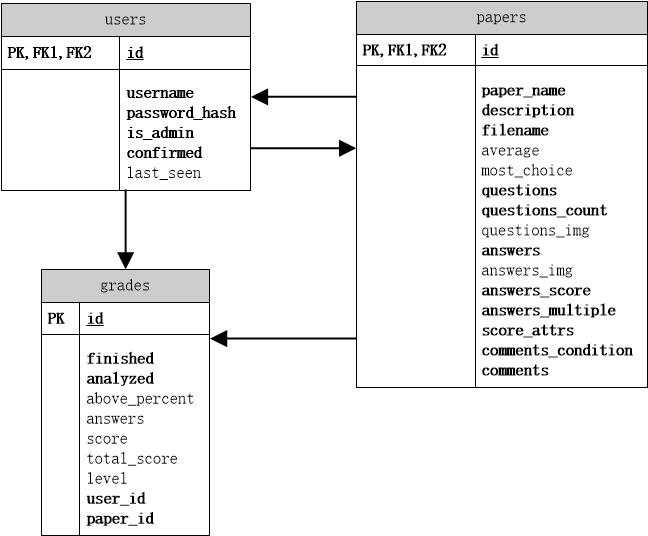
\includegraphics[width=1.0\linewidth]{figure/entity_relationship}
	\caption{数据库关系}
	\label{fig:entity_relationship}
\end{figure}

\subsection{一对多关系}

如图中,用户表和成绩表,试卷表和成绩表之间都为一对多关系。SqlAlchemy中可以方便的通过relationship和foreignKey进行设置一对多关系。

\begin{lstlisting}[language=C]
class User(Model):
  ...
  grades = relationship("Grade", backref="user", lazy="dynamic",
  cascade="all, delete-orphan", passive_deletes=True)
  
class Paper(Model):
  ...
  grades = relationship("Grade", backref="paper", lazy="dynamic",
  cascade="all, delete-orphan", passive_deletes=True)
  
class Grade(Model):
  ...
  user_id = Column(Integer, ForeignKey("users.id",
  ondelete="CASCADE"))
  paper_id = Column(Integer, ForeignKey("papers.id",
  ondelete="CASCADE"))
\end{lstlisting}

\begin{center}
	{\small 建立用户和成绩,试卷与成绩之间的一对多关系}
\end{center}

relationship的这一端代表着1的这一端,backref传入的是在Grade对象下如何访问User或者Paper对象,lazy代表如何访问这个对象,一对多之间的关系通过外键的形式进行设置,比如users.id代表着是users这张表中的id作为外键。同时外键的字段设置需要和做外键的字段类型一模一样,否则会报错。

\begin{enumerate}
\item select,默认选项,直接查找出所有对象,例如user.grades直接通过列表列出所有该用户下的grade
\item dynamic返回的是一个查询集,例如 users.grades.filter\_by(...)返回的是一个查询集可以进行筛选操作。
\item joine类似于select,但是seletc在查询的过程中需要查询两个表,而joined是建立一个新的连结表进行查询,在数额大的情况下使用joined能节省不少性能。
\end{enumerate}

\begin{center}
	{\small lazy选项}
\end{center}

SqlAlchemy作为最强大的ORM工具当然不只是定义关系,还有就是定义实体不存在的时候如何处理与其相关的数据,加入一个用户被删除了,那么于其关联的成绩也应该要全部删除,而不是作为冗余数据存在数据库中,一套试卷被删除了同理。那么cascade就是干这个事情的。

\begin{enumerate}
\item save-update,默认选项,添加一条数据的时候会把其他和它相关的数据都添加到数据库中。
\item merge,默认选项,合并一个对象的时候会将使用了relationship相关联的对象也进行merge操作。
\item expunge,移除操作的时候,会将相关联的对象也进行移除,这个操作只是从session中删除,而不是从真正的数据库中删除。
\item all,包含上面所有的选项。
\item delete-orphan,删除相关的孤儿数据。
\label{cascade选项}
\end{enumerate}

\begin{center}
	{\small cascade选项}
\end{center}

对应的要在多的那一端设置ondelete属性。

至此一对多的关系就设置好了,使用Flask-Migrate升级数据库的时候可以自动检测相关外键的设置然后更新数据库。

\subsection{多对多关系}

\begin{figure}[thbp!]
	\centering
	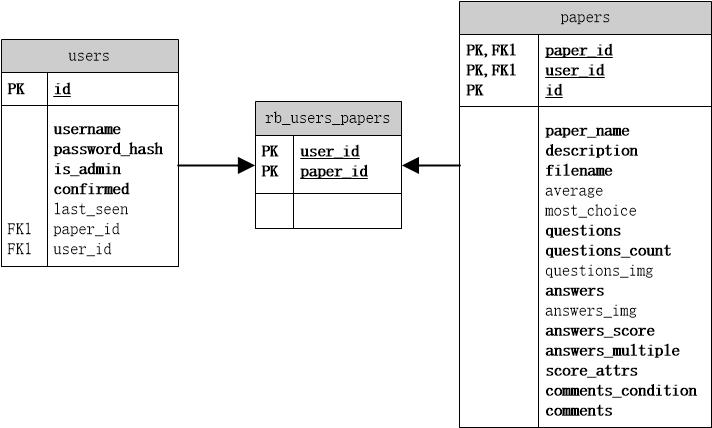
\includegraphics[width=1.0\linewidth]{figure/rb_users_papers}
	\caption{多对多关系}
	\label{fig:rb_users_papers}
\end{figure}

一个用户可以做多张试卷,一张试卷也可以有很多用户来做。这就是一个多对多关系。多对多关系中,需要一个额外的连接表来做查询。

\begin{lstlisting}[language=C]
class User(Model):
  ...
  papers = relationship("Paper", secondary=rb_users_papers,
  lazy="dynamic")

class Paper(Model):
  ...
  users = relationship("User", secondary=rb_users_papers,
  lazy="dynamic")

// 连接表
rb_users_papers = Table(
  "rb_users_papers",
  Column("user_id", Integer, ForeignKey("users.id"),
  primary_key=True),
  Column("paper_id", Integer, ForeignKey("papers.id"),
  primary_key=True)
)
\end{lstlisting}

\begin{center}
	{\small 多对多关系代码}
\end{center}

上面的代码说明了users表和papers表之间是通过一个rb\_users\_papers进行连接查询的,同时连接表中的每个字段都需要与原字段的属性相同。在原表中的relationship中需要设置secondary属性来进行使用连接表的查询。使用连接表进行连接的两个表,任何一条记录被删除以后相关的连接表记录也会被删除,当然也可以设置与其关联的记录也被删除,但在此处的情况不适合这样做,试想一下,如果一个用户记录被删除了,那么该用户做过所有的试卷记录也会被删除,别人就无法做了,这样是非常的不合适的情况。

数据库的设计是一个完善的软件系统必备也是最重要的一个阶段,一个好的数据库设计能让一个系统的性能良好、易于维护、易于拓展。有些人可能会觉得直接手写sql更加灵活和方便,但是如果作为一个多人维护开发的系统来说,每个人都有自己写sql的习惯,会让项目代码水平层次不齐难于维护,这时候就要使用SqlAlchemy这种工具了,通过一种OOP的方式来进行数据库的管理。